\section{Introduction}
One of the challenges in 3D shape processing concerns the question of representation.
Shapes are typically represented as triangle meshes or point clouds in computer graphics applications due to their simplicity and light-weight nature.
At the same time an increasing number of robotic and remote-sensing applications are deploying sensors that directly collect point-cloud representations of the environment. Hence architectures that efficiently operate on point clouds are becoming increasingly desirable.

On the other hand the vast majority of computer vision techniques rely on grid-based representation of 3D shapes for analyzing and generating them. 
These include multiview representations that render a shape from a collection of views~\cite{qi2016volumetric,mvcnn,Soltani17} or voxel-based representations~\cite{wu20153d,Huang:PCL,voxnet,BrockLRW16,3dgan} that discretize point occupancy onto a 3D grid. 
Such representations allow the use of convolution and pooling operations for efficient processing. 
However, voxel-representations scale poorly with resolution and are inefficient for modeling surface details.
Even multiscale or sparse variants~\cite{fpnn,Riegler2017CVPR,hie3dcnn} incur relatively high processing cost.
Image-based representations, while more efficient, are not effective at modeling shapes with concave or filled interiors due to self occlusions.
Moreover, generating shapes as a collection of views requires subsequent reasoning about geometric consistency to infer the 3D shape, which can be challenging.


The main contribution of our work is a multiresolution tree network capable of both recognizing and generating 3D shapes directly as point clouds.
An overview of the network and how it can be applied to different applications are shown in Figure~\ref{fig:multires-abs}.
Our approach represents a 3D shape as a set of locality-preserving 1D ordered list of points at multiple resolution levels. 
We can obtain such a ordering by using space-partitioning trees such as kd-tree or rp-tree.
Feed-forward processing on the underlying tree can be implemented as 1D convolutions and pooling on the list.
However, as our experiments show, processing the list alone is not sufficient since the 1D ordering distorts the underlying 3D structure of the shape. 
To ameliorate this problem we employ a multi-grid network architecture~\cite{multigrid} where the representation at a particular resolution influences feed-forward processing at adjacent resolutions.
This preserves the locality of point in the underlying 3D shape, improves information flow across scales, enables the network to learn a coarse-to-fine representation, and results in faster convergence during training.
Our network outperforms existing point-based networks~\cite{pointnet,Klokov_2017_ICCV,pointnet2} that operate on position ($xyz$) information of points. Specifically, it obtains \textbf{91.7\%} accuracy on the ModelNet40 classification task,
while remaining efficient.
It also outperforms similar graph networks that do not maintain multiresolution representations.

Our multiresolution decoders can be used for directly generating point clouds.
This allows us to incorporate order-invariant loss functions, such as Chamfer distance, over point clouds during training. 
Moreover it can can be plugged in with existing image-based encoders for image-to-shape inference tasks.
Our method is able to both preserve the overall shape structure as well as fine details. 
On the task of single-image shape inference using the ShapeNet dataset, our approach outperforms existing voxel-based~\cite{choy20163d}, view-based~\cite{lin2018learning}, and point-based~\cite{fan2016point} techniques.

Finally, the combined encoder-decoder network can be used for unsupervised learning of shape representations in a variational autoencoder (VAE) framework. The features extracted from the encoder of our VAE (trained on the unlabeled ShapeNet dataset) leads to better shape classification results (\textbf{86.4\%} accuracy on ModelNet40) compared to those extracted from other unsupervised networks~\cite{3dgan}.

\begin{figure*}[t!]
\centering
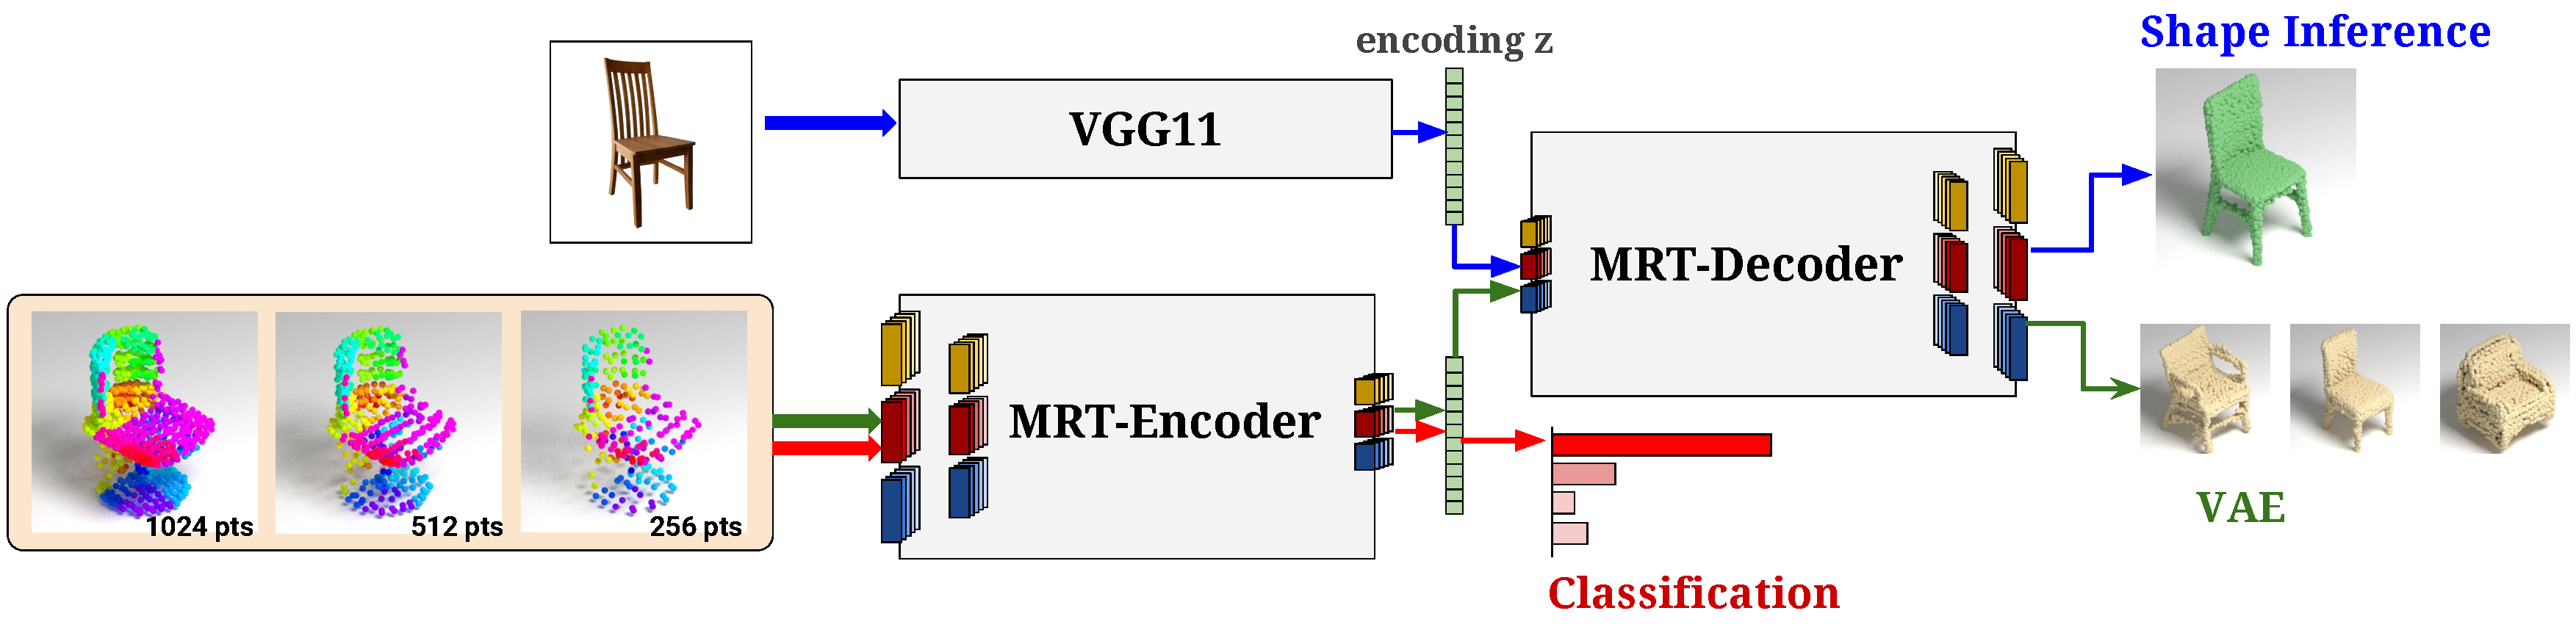
\includegraphics[width=1.0\linewidth]{MRTNet/imgs/visabstract1.pdf}
\vspace{-20pt}
	\caption{\small \label{fig:multires-abs}
  Overview of \mrtnet. On the left, the MRT-Encoder takes as input a 1D ordered list of points and represents it at multiple resolutions. Points are colored by their indices in the list. On the right, the MRT-Decoder directly outputs a point cloud. Our network can be used for several shape processing tasks, including classification (red), image-to-shape inference (blue), and unsupervised shape learning (green). Refer to Fig.~\ref{fig:multires-arch} for details on the encoder and decoder.}
\vspace{-16pt}
\end{figure*}





